% Layout/style adapted from OpenTikZ flowchart template (CC0).
% Source revision 359befbf8e8af7ce08e7e387b2c2a198e0ca735d.
% New generic conditional rectified-flow topology, not a particular published method.
\documentclass[tikz,border=10pt]{standalone}
\usepackage{amsmath,amssymb}
\usetikzlibrary{positioning,arrows.meta,calc,fit,backgrounds}
\definecolor{otblue}{HTML}{0072B2}\definecolor{otorange}{HTML}{E69F00}
\definecolor{otteal}{HTML}{009E73}\definecolor{otpurple}{HTML}{9C6194}
\definecolor{otgray}{HTML}{5A5A5A}
\def\boxW{3.0cm}\def\gapX{4.3}\def\conditionLabel{LQ observation $c$}
\begin{document}
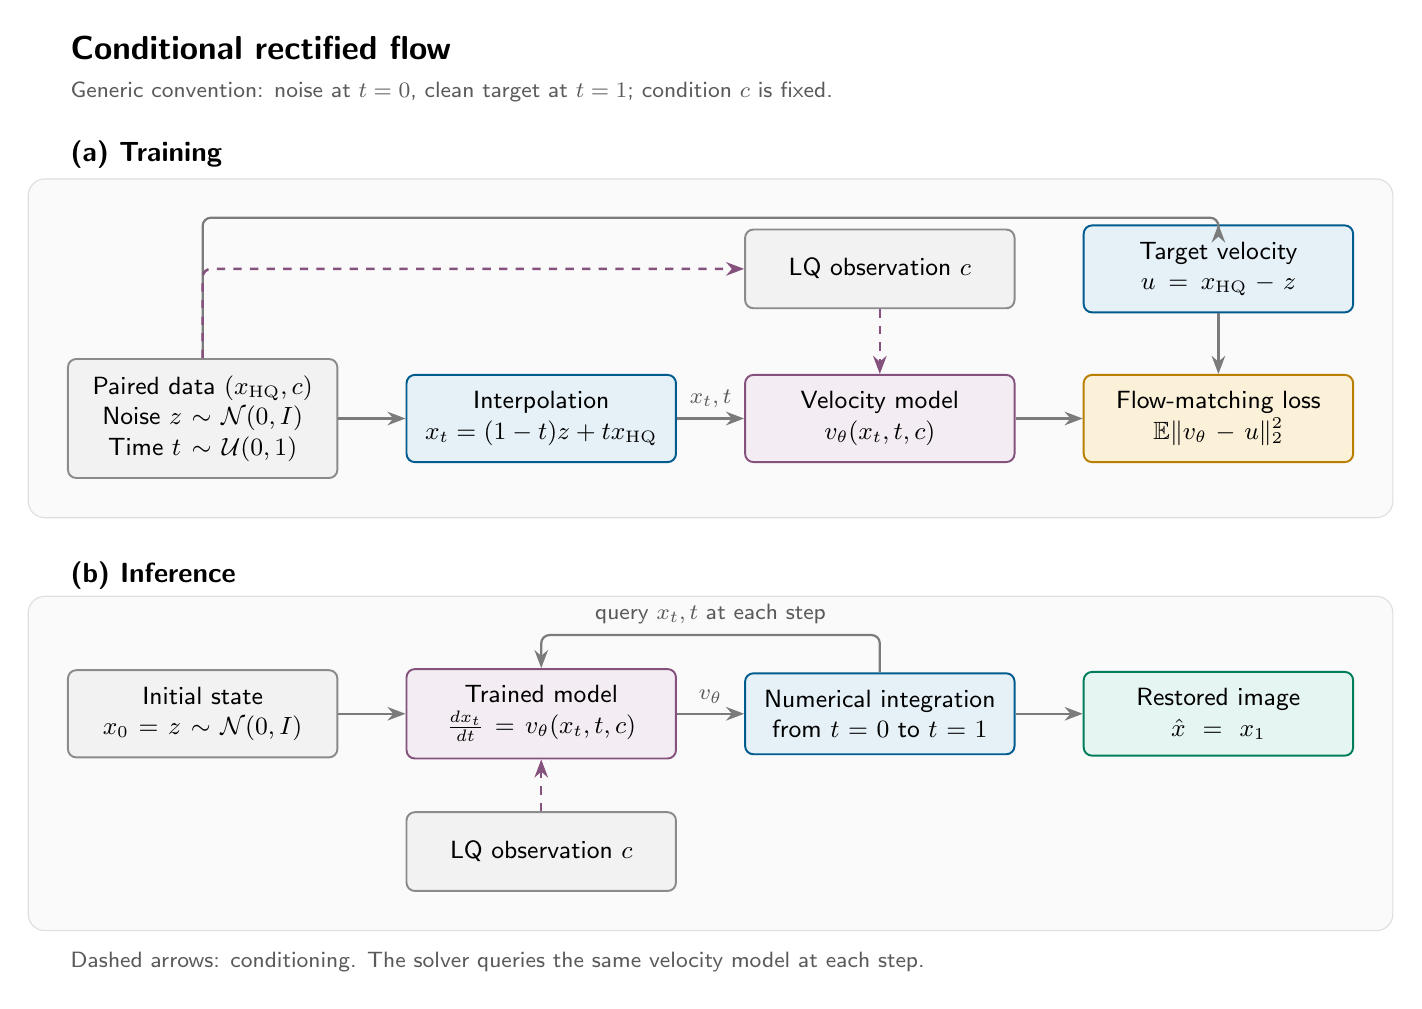
\begin{tikzpicture}[
 >={Stealth[length=2.3mm]},font=\sffamily\small,
 base/.style={line width=.7pt,align=center,text width=\boxW,minimum height=1.0cm,inner sep=6pt,rounded corners=3pt},
 data/.style={base,draw=otgray!70,fill=otgray!8},
 process/.style={base,draw=otblue!80!black,fill=otblue!10},
 model/.style={base,draw=otpurple!85!black,fill=otpurple!12},
 loss/.style={base,draw=otorange!80!black,fill=otorange!15},
 flow/.style={draw=otgray!80,line width=.8pt,->},
 condition/.style={draw=otpurple!85!black,line width=.9pt,dashed,->},
 elabel/.style={font=\sffamily\footnotesize,text=otgray},
 panel/.style={draw=otgray!20,fill=otgray!3,rounded corners=6pt,inner sep=14pt}]
\node[font=\sffamily\bfseries\large,anchor=west] at (-1.8,4.7) {Conditional rectified flow};
\node[elabel,anchor=west] at (-1.8,4.15) {Generic convention: noise at $t=0$, clean target at $t=1$; condition $c$ is fixed.};
\node[font=\sffamily\bfseries,anchor=west] at (-1.8,3.35) {(a) Training};
\node[data] (train_data) at (0,0) {Paired data $(x_{\rm HQ},c)$\\Noise $z\sim\mathcal N(0,I)$\\Time $t\sim\mathcal U(0,1)$};
\node[process] (interpolate) at (\gapX,0) {Interpolation\\$x_t=(1-t)z+t x_{\rm HQ}$};
\node[model] (velocity) at (2*\gapX,0) {Velocity model\\$v_\theta(x_t,t,c)$};
\node[loss] (objective) at (3*\gapX,0) {Flow-matching loss\\$\mathbb E\|v_\theta-u\|_2^2$};
\node[data] (train_condition) at (2*\gapX,1.9) {\conditionLabel};
\node[process] (target) at (3*\gapX,1.9) {Target velocity\\$u=x_{\rm HQ}-z$};
\draw[flow] (train_data)--(interpolate);
\draw[flow] (interpolate)--node[above,elabel] {$x_t,t$}(velocity);
\draw[flow] (velocity)--(objective);
\draw[condition] (train_condition)--(velocity);
\draw[flow] (target)--(objective);
% The target and interpolant use the same x_HQ,z sample; the paired condition is explicit.
\draw[flow,rounded corners=3pt] (train_data.north) -- (0,2.55) -- (3*\gapX,2.55) -- (target.north);
\draw[condition,rounded corners=3pt] (train_data.north) -- (0,1.9) -- (train_condition.west);
\node[font=\sffamily\bfseries,anchor=west] at (-1.8,-2.0) {(b) Inference};
\node[data] (initial) at (0,-3.75) {Initial state\\$x_0=z\sim\mathcal N(0,I)$};
\node[model] (ode) at (\gapX,-3.75) {Trained model\\$\frac{d x_t}{dt}=v_\theta(x_t,t,c)$};
\node[process] (solver) at (2*\gapX,-3.75) {Numerical integration\\from $t=0$ to $t=1$};
\node[data,draw=otteal!80!black,fill=otteal!10] (output) at (3*\gapX,-3.75) {Restored image\\$\hat x=x_1$};
\node[data] (infer_condition) at (\gapX,-5.5) {\conditionLabel};
\draw[flow] (initial)--(ode);
\draw[flow] (ode)--node[above,elabel] {$v_\theta$}(solver);
\draw[flow,rounded corners=3pt] (solver.north) -- (2*\gapX,-2.75) -- (\gapX,-2.75) -- (ode.north);
\node[elabel] at (1.5*\gapX,-2.48) {query $x_t,t$ at each step};
\draw[flow] (solver)--(output);
\draw[condition] (infer_condition)--(ode);
\node[elabel,anchor=west] at (-1.8,-6.9) {Dashed arrows: conditioning. The solver queries the same velocity model at each step.};
\coordinate (query_lane) at (\gapX,-2.75);
\begin{scope}[on background layer]
 \node[panel,fit={(train_data)(interpolate)(velocity)(objective)(target)(0,2.55)}] {};
 \node[panel,fit={(initial)(ode)(solver)(output)(infer_condition)(query_lane)}] {};
\end{scope}
\end{tikzpicture}
\end{document}
